% =============================================================================
\section{The substrate}\label{sec:substrate}
% =============================================================================

\subsection{Events, order and number}

The primitive objects are \emph{events}. An event carries no position, duration, mass or charge;
everything is relational. Events are connected by a relation of influence $\prec$ that is
\begin{itemize}
\item \emph{transitive}: $u\prec v$ and $v\prec w$ imply $u\prec w$;
\item \emph{acyclic}: $u\prec v$ and $v\prec u$ never hold together (no closed causal loops);
\item \emph{locally finite}: between any two events there are finitely many others.
\end{itemize}
A set with such a relation is a causal set~\cite{Bombelli1987,Surya2019}. Two derived notions carry
most of the physics:
\begin{itemize}
\item the \emph{interval} $I(u,v)=\{w: u\prec w\prec v\}$ and its number of elements $n(u,v)$;
\item the \emph{chains} $u\prec w_1\prec\dots\prec v$; the length of the longest chain between $u$ and
  $v$ is a discrete proper time.
\end{itemize}

When the causal set is faithfully embedded in a Lorentzian manifold $(M,g)$, the relation $\prec$ is
the causal order of $g$ and the number of elements in a region is, on average, $\rho$ times its
spacetime volume. The order fixes the metric up to a local scale; the number fixes the scale.
The standard realisation is a \emph{sprinkling}: a Poisson process of density $\rho$ per unit proper
volume, with the relation inherited from the light cones of $g$. A sprinkling is statistically
invariant under Lorentz transformations: there is no preferred frame in which it looks different
from any other.

\subsection{Why the substrate must be Lorentz invariant}\label{sec:why-lorentz}

A natural alternative is a graph in which each event has at most $K_0$ relations, locality is
distance in the graph and time is the count of updates. Such a substrate has a rest frame. A Lorentz-invariant discrete structure cannot have it: in a sprinkling every event is related
to infinitely many others along its light cone (finitely many only because a simulated region has a
wall), and no Lorentz-invariant rule can select a finite set of neighbours
locally~\cite{BombelliHensonSorkin2009}. Finite degree and Lorentz invariance of the substrate
exclude each other.

There are two options. (A) A Lorentz-invariant substrate: relativity comes for free and
non-locality is unavoidable. (B) A substrate with a rest frame: Lorentz invariance must emerge for
observers with extreme precision, and small violations at the discreteness scale tend to be
amplified by quantum corrections. The tests of the laboratory support (A)
(Appendix~\ref{app:lab}):
\begin{itemize}
\item the degree of an event grows with the number of events in the region; a bound $K_0$ does not
  hold (F0.3);
\item capacity limits the \emph{flow} through an event, not the number of its relations (F1.8;
  supported, but not robust to the seed);
\item local growth rules of the finite-degree type produced no manifold-like order (0 of 7 rules,
  F6.1) and no three-dimensional space (F6.2).
\end{itemize}
The substrate of Causal Physics is therefore a causal set. Capacity survives as a bound on the flow that an event
can carry (Part~\ref{part:axioms}).

\subsection{Non-locality}

Because every event is related to events arbitrarily far away along its light cone, local
differential operators have no direct discrete analogue. The causal set d'Alembertian of Benincasa
and Dowker~\cite{BenincasaDowker2010}, in its smeared form due to Sorkin~\cite{Sorkin2007}, sums
over the whole causal past of an event with weights that depend on the number of elements in each
interval. The smearing introduces a non-locality scale
\begin{equation}
  \ell_k=(\epsilon\rho)^{-1/D},
\end{equation}
where $D$ is the spacetime dimension and $0<\epsilon\le1$ the smearing parameter. For $\epsilon=1$,
$\ell_k$ is the discreteness scale itself; for small $\epsilon$ it is larger. The operator is defined in
Sec.~\ref{sec:bd}; its non-locality is a physical property of the substrate, and one of the results of
this paper (Part~\ref{part:geometric}) is a non-local term in the action that it implies.

% =============================================================================
\section{Reading geometry from the order}\label{sec:reading}
% =============================================================================

A theory in which geometry is emergent must say how geometry is read. For a weak static field in
isotropic coordinates,
\begin{equation}\label{eq:weakmetric}
  \dd s^2=-e^{2\phi}\,\dd t^2+e^{-2\psi}\,\dd\vec x^2,\qquad \gamma=\psi/\phi,
\end{equation}
($\phi$ the clock potential, $\psi$ the spatial potential, $\gamma$ the post-Newtonian parameter),
three quantities of the order determine both potentials:

\begin{center}
\begin{tabular}{lll}
\toprule
quantity of the order & what it measures & weak-field value\\
\midrule
clocks: elements of a small interval at rest & proper time & $\phi$\\
the boundary of the relation & speed of the causal cone $c$ & $\phi+\psi$\\
density of elements per coordinate volume & $\sqrt{-g}$ & $\phi-d_s\psi$\\
\bottomrule
\end{tabular}
\end{center}
($d_s$ is the number of spatial dimensions.) Any two of the three determine $\gamma$; the third is a
consistency check that the order is metric at all.

\paragraph{The blind instrument.} The laboratory built an instrument that receives only the events,
the relation and the fundamental density, not the metric, and reads $\gamma$ along two independent
paths: (A) cones and density, (B) clocks and cones. It was calibrated on orders sprinkled into
metrics with known $\gamma$ (K.16b in 2+1, K.16c in 3+1). In 2+1, for a field
$\phi=-0.1\,e^{-r^2/128}$, it returns $-1.000\pm0.001$ for $\gamma=-1$, $-0.04\pm0.02$ for $\gamma=0$
and $+0.92\pm0.03$ for $\gamma=+1$. In 3+1 it returns $-1.001\pm0.001$, $0.33\pm0.04$ and
$0.99\pm0.05$ for $\gamma=-1,\ 1/3,\ +1$. For fields weaker than $|\phi|\sim0.03$ the instrument is
unreliable; all tests that use it work with $|\phi|\sim0.1$. The instrument uses coordinates and
the known density as a declared readout; a coordinate-free reading (radar echoes) is a planned
improvement. Figure~\ref{fig:blind} shows the calibration and the potentials read by radius.

\begin{figure}[t]
  \centering
  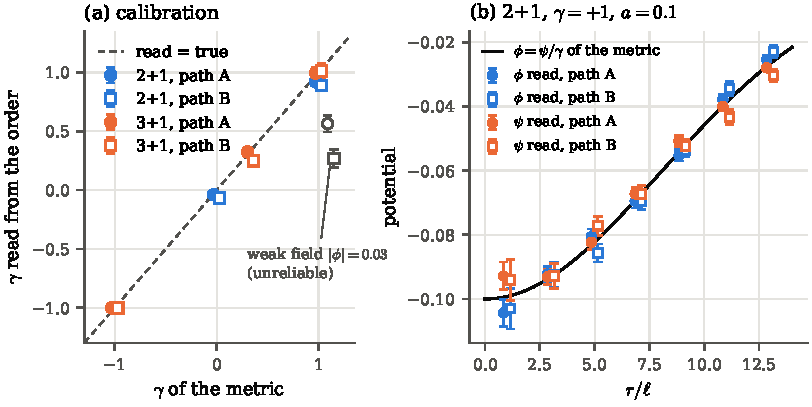
\includegraphics[width=\textwidth]{figures/fig_blind.pdf}
  \caption{The blind instrument (K.16b, 2+1; K.16c, 3+1). (a) $\gamma$ read from orders sprinkled into metrics of known
$\gamma$, along path A (cones and density, filled) and path B (clocks and cones, open); grey: the weak field
$|\phi|=0.03$, where the instrument is unreliable. (b) The potentials read by radius for $\gamma=+1$ in 2+1
($a=0.1$, $\psi=\phi$) against the profile of the metric. Bars: $\pm1$ standard error over 32 (2+1) and 16 (3+1)
sprinklings.}\label{fig:blind}
\end{figure}

\paragraph{Other instruments.} The clock rate $\Pi$ can be read back from the density of chains
(K.3); the causal front of a source measures the Shapiro delay to within $2\%$ of the general
relativistic value (K.2); and the number of ``horizon molecules''~\cite{DouSorkin2003,Barton2019}
measures the area of a horizon in flat space in 1+1, 2+1 and 3+1 dimensions and its \emph{proper} area in
a conformally flat geometry, with the exponent of the proper-area law $1.96\pm0.06$ against $2$ in 3+1 (K.14). The last instrument is the entropy meter of the
thermodynamic route of Sec.~\ref{sec:jacobson}.

% =============================================================================
\section{Matter as flows}\label{sec:flows}
% =============================================================================

\subsection{Flow and its conservation}

Matter in Causal Physics is a persistent pattern of events. Its simplest model is a \emph{flow}: a
non-negative quantity $F$ transported from events to their successors along the relations of the
order and conserved at every event (Axiom~\ref{ax:continuity}). A steady source then obeys Gauss's
law: the flow through any closed surface around it equals the source, $J/S=1.003$--$1.004$ in 2+1 and
3+1 with up to $2.6\times10^5$ events, against $0.77$--$0.88$ for a model without conservation (F1.1).

\subsection{A flow carries its four-velocity}\label{sec:inertia}

How the flow is shared among successors decides whether anything localised can exist. If an event
divides its flow equally among all successors, a source spreads at $0.77c$. If each step takes its
direction from the previous step, the memory decays within a few relations (a single relation turns
the direction by $0.45$--$0.52$ in rapidity) and the flow spreads at $\sim0.4c$. If the flow carries
its timelike direction as an internal \emph{state}, the bundle stays at the world line of its
source, $v_s=0.054\pm0.006\,c$ (F3.6, replicated). A source moving at $0.5c$ is followed: the
bundle is at rest in the frame of the source ($+0.008\pm0.004$ against the alternative $-0.5$), and
its width evolves as for a source at rest, as the principle of relativity requires. Recomputing the
rule in a frame boosted by $0.6c$ gives the same choice at every event.

This was the first result of the laboratory that had not been put into the rule. It shows that
localisation on a Lorentz-invariant substrate requires a memory of direction, and that the memory
is inertia: a flow carries momentum.

\subsection{The energy--momentum tensor of flows}\label{sec:tab}

With a four-velocity $u^a$ per carrier, the flows have an energy--momentum tensor
\begin{equation}\label{eq:Tab}
  T^{ab}=\frac{1}{\Delta V_4}\sum F\,u^au^b\,\tau ,
\end{equation}
summed over the relations in a spacetime cell of volume $\Delta V_4$, with $\tau$ the proper duration
of each relation. The laboratory measures it correctly for dust, for two counter-streaming
populations and for an isotropic gas (K.15): for a beam at $v=0.6$ the cell values are
$E/e_0=\gamma_v^2=1.5625$ ($e_0$ the rest-frame energy density), $|q|/E=v$, $S_{xx}/E=v^2$ without scatter, and the pressure of an
isotropic gas is reproduced to within $7\%$. When flows of different directions merge, the rule
$F=|P|$ (the merged flow is the length of the summed four-momentum) conserves four-momentum
exactly ($6\times10^{-17}$), while the earlier rule ``flow $=$ sum of flows'' loses up to $2\%$ of
the energy. Conservation $\partial_aT^{ab}=0$ is the condition without which a tensor coupling to
gravity is inconsistent (Part~\ref{part:geometric}).

\subsection{Contact: flows that meet stick}\label{sec:contact}

Every event passes its whole flow to one successor, so two flows interact by contact only if their chains choose
the same events; a priori they might cross each other without interacting. They do not. Two flows sent head-on
at $\pm0.6$ merge on contact: after the crossing $77$--$82\%$ of the flow is on events that carry both
($0.821\pm0.013$ in 2+1, $0.774\pm0.008$ in 3+1), the merged flow is at rest in the centre-of-momentum frame
($-0.008\pm0.013$ and $-0.003\pm0.011$), its rest mass exceeds the sum of the merged rest masses by up to the
Lorentz factor ($1.216$ against $\gamma=1.25$ for equal parts), and no flow reverses its motion. Flows displaced
so that they do not touch do not merge (F4.1, \verdict{passed} in both dimensions). Contact between flows is a
perfectly inelastic collision: momentum is shared, kinetic energy becomes rest mass, and the inertia of the merged
flow is its energy. The rule has no elastic channel; elastic scattering of matter must come from fields or from
bound structure, which the model does not yet have.

% =============================================================================
\section{The action of a flow}\label{sec:action}
% =============================================================================

The Causal Resistance Functional $\mathcal R=\sum_v Z_v\Delta\tau$ (impedance $Z_v$ times the causal
update increment) is the action of a flow along its history. Its content depends on what
$\Delta\tau$ is. Here $\Delta\tau$ is the proper time between successive events of the flow, as counted by the order (the length of the longest chain, or equivalently the number of
elements of a small interval). Then, for a flow with mass $m$,
\begin{equation}\label{eq:A6}
  S_m=-\sum m\,\Delta\tau \;\longrightarrow\; -m\!\int\!\dd\tau ,
\end{equation}
the action of a free particle (Axiom~\ref{ax:action}).

Two consequences follow without further assumptions.
\begin{enumerate}
\item \textbf{On a fixed order the geometry of motion is conformal.} If clocks are slowed by a
  factor $\Pi$ but the order is the flat one, the action is
  $\int\Pi\sqrt{\dd t^2-\dd\vec x^2}$, the geodesic action of the conformally flat metric
  $\Pi^2\eta$. Maximal chains on sprinklings follow exactly these geodesics (F2.2, F2.4, F2.5 in
  3+1). But null geodesics of a conformally flat metric are straight: light is not deflected,
  $\gamma=-1$.
\item \textbf{The coupling to the order is through $T_{ab}$.} For a small change of the geometry
  $g=\eta+h$ the proper time changes by $\delta\tau=-\tfrac12h_{ab}u^au^b\tau$, so
  \begin{equation}\label{eq:dSdh}
    \frac{\delta S_m}{\delta h_{ab}}=\tfrac12\,T^{ab}.
  \end{equation}
  The order ``sees'' a flow only through $u^au^b$, that is in the rest frame of the flow, and
  contributions of different flows add. These two facts are the substrate rule of
  Sec.~\ref{sec:rule}, derived rather than assumed.
\end{enumerate}

% =============================================================================
\section{How the order responds to matter}\label{sec:response}
% =============================================================================

If the order near matter were fixed, gravity would be the scalar Nordstr\"om class and light would
not bend. Gravity in Causal Physics therefore \emph{changes the causal order}: near matter causal cones
narrow and events become denser. Causality itself is untouched: there are no closed loops and the
flow is conserved. How much the cones narrow relative to how much the density grows is a single
number, and it is $\gamma$:

\begin{center}
\begin{tabular}{llll}
\toprule
response of the order & cones & density & $\gamma$\\
\midrule
fixed order & unchanged & unchanged & $-1$\\
cones narrow, events kept (capacity) & narrower & unchanged & $1/d_s$\\
causal throughput conserved & narrower & denser, $\rho_c\,c=\text{const}$ & $2/(d_s-1)$\\
general relativity (3+1) & $c=e^{2\phi}$ & $\rho_c=e^{-2\phi}$ & $1$\\
\bottomrule
\end{tabular}
\end{center}

\paragraph{The throughput principle.} Where the substrate slows the propagation of influence, events
become denser in such a way that the number of events crossed by a light front per unit time and
area stays the same,
\begin{equation}\label{eq:throughput}
  q=\rho_c\,c=\text{const}.
\end{equation}
This is the continuity law of traffic (flow $=$ density of cars $\times$ their speed) and of any conserved current through a
constriction. It makes precise the picture of $c$ as the maximal congestion-free throughput of the
substrate, with an effective speed that falls where the substrate is loaded.
With the dictionary of Sec.~\ref{sec:reading}, $\ln(\rho_c c)=2\phi-(d_s-1)\psi$, so
\begin{equation}
  \gamma=\frac{2}{d_s-1},
\end{equation}
which is $\gamma=1$ exactly in three spatial dimensions. In 3+1 the principle together with a clock
rate $\Pi$ fixes the metric completely, $\dd s^2=-\Pi^2\dd t^2+\Pi^{-2}\dd\vec x^2$, with
$c_{\rm eff}=\Pi^2$ and $\rho_c=\Pi^{-2}$.

\paragraph{Tests.} The three responses were built as discrete orders and read with the blind
instrument.
\begin{itemize}
\item \emph{Cones only} (F7.1a, 2+1): $\gamma=0.47\pm0.03$ and $0.43\pm0.03$ against $1/2$,
  independent of the strength of the coupling, as derived before the run: narrowing the cones without
  adding events cannot give $\gamma=1$. In 3+1 the same rule reads $0.35\pm0.02$ against $1/3$.
\item \emph{Throughput} (F7.1b, 2+1): $\gamma\approx1.85\pm0.1$ against the prediction $2$, in two
  independent runs; formally \verdict{undecided} because the two reading paths deviate in
  opposite directions by $0.1$--$0.2$.
\item \emph{Throughput} (F7.1c, 3+1): $\gamma=1.000\pm0.045$ (path A) and $0.972\pm0.074$ (path B);
  replication $0.948\pm0.047$ and $0.979\pm0.058$. The raw readings agree with the prediction, and
  the orders are metric (the two paths agree). Formally the test is \verdict{undecided}: it compares
  with an exact $\gamma=1$ metric read by the same instrument in the same run, and in path B that
  control read low ($0.78\pm0.08$ and $0.90$). The design left too little room for the statistical
  error of the comparison; the verdict stands as recorded.
\end{itemize}
All readings, with the controls, are shown in Fig.~\ref{fig:response}.

\begin{figure}[t]
  \centering
  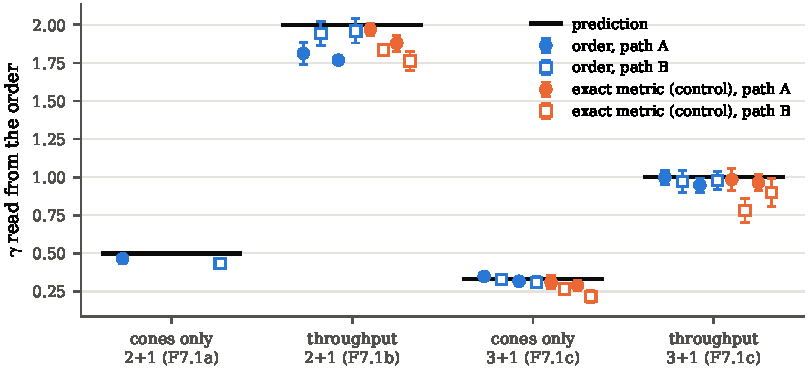
\includegraphics[width=\textwidth]{figures/fig_response.pdf}
  \caption{$\gamma$ of the responses of the order (F7.1a; F7.1b and F7.1c, two independent runs each), path A (filled) and
path B (open), against the prediction (black bar). Orange: orders sprinkled into the exact metric with the
predicted $\gamma$ and read by the same instrument in the same run (the controls of F7.1b and F7.1c); in 3+1
path B of the control reads low, which leaves F7.1c undecided. Bars: $\pm1$ standard error.}\label{fig:response}
\end{figure}

\paragraph{What this does and does not show.} The tests show that a discrete order built according
to the throughput principle has the geometry of $\gamma=1$ in 3+1. They do not show why the
substrate conserves its throughput. Part~\ref{part:geometric} answers that question at the linear
order: the principle is the linearised coupling of general relativity, and it follows from an action
of the order with the Einstein--Hilbert stiffness, which the expected Benincasa--Dowker action has.

% =============================================================================
\section{Free fall in the order}\label{sec:fall}
% =============================================================================

The order of Sec.~\ref{sec:response} carries gravity: its longest chains between two fixed events sag
towards the mass. A separate question is whether matter, moved by a local rule that reads only the
order, falls. Such a rule contains no bending law and no field; the fall has to come from inertia and from
the order itself.

\paragraph{Set-up.} The 2+1 throughput order of F7.1b with $\sigma_0=0.45$: density $e^{\sigma}$,
cones $e^{-\sigma}$, $\sigma=\sigma_0\exp(-r^2/2w^2)$, $w=8$. With the dictionary of
Sec.~\ref{sec:reading} its clock potential is $\phi=-\sigma/3$ ($\gamma=2$), which predicts the Newtonian
acceleration $a_{\rm pred}$ of a slow body. A history is continued as a longest chain: from its last event
$v$, with the event $p$ eight steps back, the rule looks at the events $q$ eight links ahead,
$L(v,q)=8$, and steps along a longest chain towards the one with the smallest $L(p,q)$, i.e.\ the
straightest continuation by the reverse triangle inequality. The reading is $R=a/a_{\rm pred}$, with $a$
from a quadratic fit of the mean radial displacement over 22 units of time. Fixed before each run: the
history falls as predicted if $\tfrac12<R\mp2\,\text{SE}<2$; in the flat order neither the histories may
drift nor the longest chains sag, and in the loaded order the longest chains must read the geometry,
$\tfrac12<R_{\max}\mp2\,\text{SE}<2$.

\paragraph{Results.}
\begin{itemize}
\item A direction carried in flat coordinates (F5.1, carried) keeps its direction and does not
  fall, $R=-0.11\pm0.04$ (the control read $R_{\max}=0.63\pm0.07$, narrowly below its band:
  \verdict{instrument failed}). A rule that keeps to the layer of the longest chains from the origin
  (F5.1, intrinsic) moves outwards, $R=-0.30\pm0.07$: \verdict{failed}.
\item The longest-chain rule started from a virtual history at rest (F5.1c) moves inwards but not with
  the Newtonian acceleration, $R=0.34\pm0.05$: \verdict{failed}. A history at rest is not a free state of
  the order.
\item The same rule started at the apex of a thrown ball (F5.1d): the history is the rising half of the
  longest chain between two events at the same place, a free state read from the order. It falls,
  $R=1.069\pm0.051$: \verdict{passed}. Flat order $R=0.15\pm0.10$; longest chains $R_{\max}=0.74\pm0.08$
  (loaded) and $0.10\pm0.12$ (flat). Fig.~\ref{fig:fall}.
\end{itemize}

\begin{figure}[t]
  \centering
  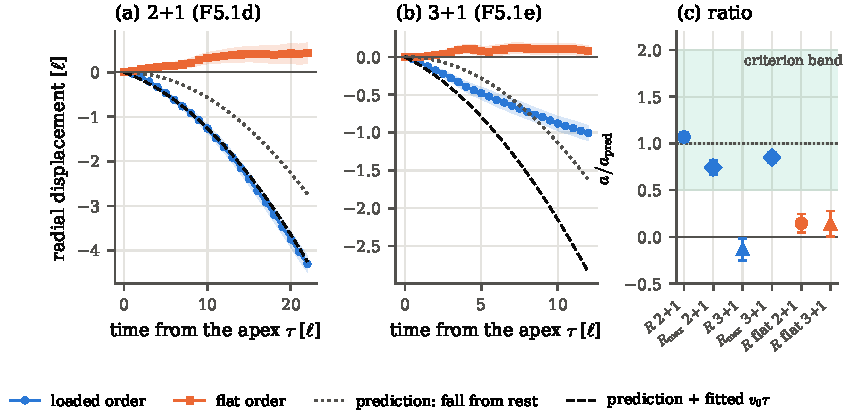
\includegraphics[width=\textwidth]{figures/fig_fall.pdf}
  \caption{Free fall from the apex (F5.1d, 2+1, 32 sprinklings per order, 40 histories each). (a) The mean
radial displacement from the apex (band $\pm1$ standard error across sprinklings) in the loaded and the flat
order; dotted: the Newtonian fall from rest at the apex radius, the prediction of the test; dashed: the same
fall with the fitted start velocity $v_0$. (b) $R=a/a_{\rm pred}$ and the control $R_{\max}$ with the
criterion band $\tfrac12<R<2$. Bars: $\pm1$ standard error.}\label{fig:fall}
\end{figure}

\paragraph{What this does and does not show.} In an order shaped by matter, a history that continues as a
longest chain falls with the Newtonian acceleration, without a bending rule, provided it starts from a
free state of the order. The limits are: one run in 2+1; the start from the apex was introduced after
F5.1c failed, with its criteria fixed before the run; the fit gives an inward start velocity
$v_0=-0.069\pm0.011$, while the rising half of the history moved outwards at $+0.026$, a jump at the apex
that the rule does not yet explain; the fall is $1.44$ times what the longest chains read of the geometry;
and the flat order drifts slightly outwards, within its tolerance. A replication, the 3+1 version and frame
dragging by a rotating source are the next tests.

% =============================================================================
\section{The Benincasa--Dowker operator and action}\label{sec:bd}
% =============================================================================

For a causal set sprinkled at density $\rho$ into a $D$-dimensional spacetime, the smeared
Benincasa--Dowker (BD) operator acting on a field $f$ is~\cite{BenincasaDowker2010,Sorkin2007,DowkerGlaser2013}
\begin{equation}\label{eq:Bdiscrete}
  (B_\epsilon f)(x)=-a_D(\epsilon\rho)^{2/D}\Big[f(x)+\sum_{y\prec x}K_\epsilon(n_{xy})\,f(y)\Big],
\end{equation}
\begin{equation}
  K_\epsilon(n)=\epsilon(1-\epsilon)^n\sum_i C_i\binom{n}{i}\Big(\frac{\epsilon}{1-\epsilon}\Big)^{i},
\end{equation}
where $n_{xy}$ is the number of elements strictly between $y$ and $x$. In 3+1 the coefficients are
$C=(-1,9,-16,8)$ and $a_4=4/\sqrt6$. Its expectation over sprinklings is
\begin{equation}\label{eq:Bexpect}
  \Ex[B_\epsilon f](x)=-a_D(\epsilon\rho)^{2/D}\Big[f(x)+\epsilon\rho\!\int_{J^-(x)}\!\!\sqrt{-g(y)}\;
    g_k\big(\epsilon\rho V(x,y)\big)f(y)\,\dd^Dy\Big],
\end{equation}
with $V(x,y)$ the proper volume of the interval and
\begin{equation}\label{eq:gk}
  g_k(w)=e^{-w}\sum_i C_i\frac{w^i}{i!}.
\end{equation}
In the continuum limit it tends to $\Box_g-\tfrac12R$ in curved
spacetime~\cite{BenincasaDowker2010,Belenchia2016}. The laboratory confirmed this limit with its own
instruments, for conformally flat geometries (K.11, K.11c) and, separately for the density part and
the cone part, for the geometry with bent light (K.13a: within $0.8$--$2.4\%$ at a field width of
$32\ell_k$).

The BD \emph{action} of a causal set is
\begin{equation}\label{eq:SBD}
  S_\BD=-\frac{2}{\rho}\sum_x (B_\epsilon 1)(x),
\end{equation}
whose expectation tends, in the continuum, to the Einstein--Hilbert action $\int\sqrt{-g}\,R$ plus
boundary terms~\cite{BuckDowkerJubbSurya2015}. In this paper the BD action is the candidate dynamics of the order. Part~\ref{part:geometric}
computes its expectation to second order in static perturbations and compares the result with the
Einstein--Hilbert value, which enters only as the normalisation of the comparison.
